\chapter{Assembly, stack và heap}

\section{Lệnh assembly cơ bản}

Các lệnh hợp ngữ xử lý trên các toán hạng. Địa chỉ của toán hạng cho biết vị trí của dữ liệu được xử lý trên bộ nhớ. Một số lệnh không yêu cầu toán hạng, một số lệnh khác lại yêu cầu 1, 2 hoặc 3 toán hạng.

Về cơ bản có 3 chế độ lập địa chỉ là:
\begin{itemize}
    \item Địa chỉ tức thời (Immediate addressing);
    \item Địa chỉ thanh ghi (Register addressing);
    \item Địa chỉ vùng nhớ (Memory addressing).
\end{itemize}

Khi lệnh có 2 toán hạng, thường thì toán hạng đầu tiên là toán hạng đích, lưu giá trị trên thanh ghi hoặc ở 1 vị trí nào đó trên vùng nhớ, còn toán hạng thứ 2 là nguồn. Nguồn thường là các hằng số (chứa trong địa chỉ tức thời) hoặc địa chỉ (trong thanh ghi hoặc bộ nhớ). Giá trị của nguồn không thay đổi sau khi tính toán.

\subsection*{Nhóm lệnh truyền dữ liệu}

\begin{itemize}
    \item \textbf{mov [đích], [nguồn]}: truyền dữ liệu (word hoặc block) từ nguồn (thanh ghi hay bộ nhớ trong) tới đích;
    \item \textbf{load [đích], [nguồn]}: đọc dữ liệu từ bộ nhớ nguồn vào thanh ghi đích;
    \item \textbf{store [đích], [nguồn]}: lưu dữ liệu từ thanh ghi nguồn vào vùng nhớ ở địa chỉ đích;
    \item \textbf{push [nguồn]}: lưu dữ liệu từ thanh ghi vào stack (thường thấy khi gọi hàm);
    \item \textbf{pop}: đưa dữ liệu từ stack vào thanh ghi.
\end{itemize}

Một số lệnh và ý nghĩa:

\begin{table}
    \centering
    \begin{tabular}{ | c | c | c | p{0.4\textwidth} | } 
    \hline
    Đích & Nguồn & Ví dụ & Ý nghĩa \\ 
    \hline
    Bộ nhớ & Thanh ghi & mov 100h, ax & Chuyển nội dung trong thanh ghi ax vào vị trí nhớ 100h \\ 
    \hline
    Thanh ghi & Bộ nhớ & mov eax, mem1 & Chuyển nội dung trong vị trí nhớ mem1 vào thanh ghi eax \\ 
    \hline
    Thanh ghi & Thanh ghi & mov eax, ebx & Chuyển nội dung trong thanh ghi ebx vào thanh ghi eax \\
    \hline
    Thanh ghi & Hằng số & mov eax, 13h & chuyển giá trị hằng 13 ở hệ hexa vào thanh ghi eax \\
    \hline
    \end{tabular}
\end{table}

\subsection*{Nhóm lệnh tính toán số học}

Các lệnh số học bao gồm phép tính cộng, trừ, nhân, chia và đảo dấu toán hạng. Trong đó toán hạng nguồn và đích có thể là các địa chỉ khác nhau nhưng phải chứa dữ liệu có cùng độ dài (ax thì tương ứng bx còn ebx không hợp lệ,......). 

\begin{example}
    Ví dụ các lệnh cộng, trừ.

    add ax, bx // ax $\leftarrow$ ax + bx

    sub cx, 15h // cx $\leftarrow$ cx - [15h]

    add ax, 15h // ax $\leftarrow$ ax + [15h]
\end{example}

Các lệnh số học cơ bản:

\begin{itemize}
    \item \textbf{add}: cộng;
    \item \textbf{addd}: cộng số có dấu chấm động, chính xác kép;
    \item \textbf{sub}: trừ;
    \item \textbf{subd}: trừ số có dấu chấm động, chính xác kép;
    \item \textbf{mul}: nhân;
    \item \textbf{div}: chia;
    \item \textbf{neg}: đảo dấu toán hạng;
    \item \textbf{inc}: tăng lên 1;
    \item \textbf{dec}: giảm đi 1.
\end{itemize}

\begin{example}
    Để cộng 2 số 5h và 3h sau đó lưu thanh ghi cx ta có thể làm như sau:

    mov ax, 5h // ax $\leftarrow$ 5h

    mov bx, 3h // bx $\leftarrow$ 3h

    add ax, bx // ax $\leftarrow$ ax + bx

    mov cx, ax // cx $\leftarrow$ ax
\end{example}

\subsection*{Nhóm lệnh logic}

Nhóm này gồm các phép tính logic not, and, or, xor và test.

\begin{itemize}
    \item \textbf{not}: đảo tất cả bit trong toán hạng (0 thành 1 và 1 thành 0);
    \item \textbf{and/or/xor}: thực hiện phép and/or/xor trên từng cặp bit trong toán hạng nguồn và đích;
    \item \textbf{test}: giống and nhưng không làm thay đổi giá trị toán hạng đầu tiên (toán hạng đích).
\end{itemize}

\subsection*{Nhóm các lệnh điều kiện và lệnh nhảy}

Nhóm lệnh điều kiện có chức năng kiểm tra điều kiện để quyết định thực hiện lệnh kế tiếp là lệnh nào, thông thường sẽ đi kèm lệnh nhảy (nhảy tới lệnh kế tiếp khi thỏa hoặc không thỏa điều kiện).

Có hai loại lệnh nhảy:

\begin{itemize}
    \item \textbf{Nhảy không điều kiện}: thực hiện bởi lệnh \textbf{jmp};
    \item \textbf{Nhảy có điều kiện}: thực hiện bởi lệnh \textbf{j$\langle$ điều kiện $\rangle$} phụ thuộc vào điều kiện được xét.
\end{itemize}

Lệnh \textbf{cmp}, là câu lệnh để thực hiện việc so sánh (compare) điều kiện.

Cú pháp là \textbf{cmp [đích] [nguồn]}, tương tự như các lệnh tính toán số học, nguồn có thể là hằng, thanh ghi, vùng nhớ, còn đích thì là thanh ghi hoặc vùng nhớ.

Thông thường, việc so sánh là để quyết định việc rẽ nhánh và nhảy đến một vị trí nào đó.

1. \textbf{Lệnh nhảy không điều kiện}. Lệnh \textbf{jmp} cho phép nhảy tới một nhãn với cú pháp là \textbf{jmp lable}

\begin{example}
    Dòng lệnh cuối là chỉ thị quay lại vòng lặp mô tả bởi nhãn LE003.
    \begin{lstlisting}
    mov ax, 8h
    mov bx, 9h
    mov cx, 0ffh
    LE003:
        add ax, 01
        sub bx, 01
        add cx, ax
        jmp LE003 
    \end{lstlisting}
\end{example}

2. \textbf{Lệnh nhảy có điều kiện}. Khi một điều kiện nhảy thỏa mãn, luồng điều khiển sẽ được đưa đến câu lệnh cần thực thi. Có nhiều loại điều kiện nhảy, ví dụ:

\begin{itemize}
    \item \textbf{je/jz}: jump equal/jump zero, nhảy khi bằng nhau/nhảy khi kết quả so sánh bằng 0;
    \item \textbf{jg/jnle}: jump greater/jump not less or equal, nhảy khi lớn hơn/nhảy khi không nhỏ hơn hoặc bằng.
\end{itemize}

\section{Stack và Heap}

Phần này sẽ sử dụng ngôn ngữ C/C++ và 1 số câu lệnh Assembly để giải thích nguyên lý của stack và heap.

Để đơn giản thì dưới đây bắt đầu với kiến trúc x86 (thanh ghi độ dài 32 bit và có tiền tố là e như eax, ebx, ...).

\subsection*{Stack}

Stack là cấu trúc dữ liệu vào sau ra trước. Khi hàm thực thi, nó sẽ tạo ra vùng nhớ stack cho bản thân nó (kể cả hàm main). Vùng nhớ này chứa các tham số truyền vào (trừ tham chiếu) và các biến cục bộ. Ta xét chương trình sau viết trên C:

\begin{lstlisting}[language=C++]
#include <stdio.h>
int m = 100;
double n = 8;
int square(int x)
{
    return x * x;
}
int cube(int x)
{
    return square(x) * x;
}
int main()
{
    int a = 4, b = 8;
    int c = square(a);
    int d = cube(b);
    return 0;
}
\end{lstlisting}

Chương trình được biên dịch thành executable file 32 bit bởi GCC phiên bản 11.4.0 bằng lệnh Linux:

\begin{lstlisting}[language=bash]
    gcc -m32 main.c -o main
\end{lstlisting}

\underline{Bước 1. Biến toàn cục}. Đầu tiên, biến toàn cục \texttt{m} và \texttt{n} sẽ được lưu trong Data Segment. 

\underline{Bước 2. Hàm \texttt{main}}. Sau đó là Stack Segment. Các chương trình C/C++ sẽ được thực thi bắt đầu từ hàm \texttt{main}. Khi hàm \texttt{main} chạy, nó tạo ra vùng nhớ cho nó, đẩy các biến \texttt{a}, \texttt{b}, \texttt{c}, \texttt{d} vào stack ngược thứ tự khai báo (hình \ref{stack:1}).

\begin{figure}[ht]
    \centering
    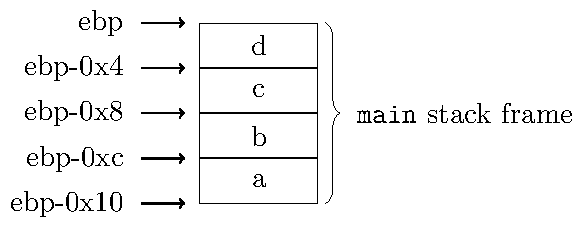
\includegraphics[page=1]{assembly/stack.pdf}
    \caption{Hàm \texttt{main}}
    \label{stack:1}
\end{figure}

Hình \ref{stack:1} có thể được giải thích khi dùng objdump ra đoạn assembly dưới đây.

\begin{lstlisting}[language={[x86masm]Assembler}]
000011c0 <main>:
    push   ebp
    mov    ebp,esp
    sub    esp,0x10
    call   1201 <__x86.get_pc_thunk.ax>
    add    eax,0x2e11
    mov    DWORD PTR [ebp-0x10],0x4
    mov    DWORD PTR [ebp-0xc],0x8
    push   DWORD PTR [ebp-0x10]
    call   118d <square>
    add    esp,0x4
    mov    DWORD PTR [ebp-0x8],eax
    push   DWORD PTR [ebp-0xc]
    call   11a2 <cube>
    add    esp,0x4
    mov    DWORD PTR [ebp-0x4],eax
    mov    eax,0x0
    leave  
    ret 
\end{lstlisting}

Biến \texttt{a} nằm ở vị trí 0x10 và biến \texttt{b} nằm ở vị trí 0xc. Vậy thì \texttt{a} nằm thấp hơn \texttt{b}. Điều này nghĩa là stack đi từ trên xuống.

Sau đó, giá trị 4 được chép qua biến \texttt{a}, giá trị 8 được chép qua biến \texttt{b}. Kế tiếp, trong hàm \texttt{main} gọi hàm \texttt{square}. Khi đó các tham số cần thiết cho hàm \texttt{square} sẽ được nạp vào stack (ở đây là biến \texttt{a} ở ebp-0x10) và hàm \texttt{square} sẽ được nạp vào stack \ref{stack:2}.

\begin{figure}[ht]
    \centering
    \includegraphics[page=2]{assembly/stack.pdf}
    \caption{Gọi hàm \texttt{square}}
    \label{stack:2}
\end{figure}

\underline{Bước 3. Gọi hàm \texttt{square}}. Hàm \texttt{square} có một tham số truyền vào là \texttt{a} ở địa chỉ ebp+0x8 (ebp mới của hàm \texttt{square}, không phải của \texttt{main}).

Ở đây, chương trình đưa giá trị 4 (ở ebp+0x8) vào thanh ghi eax và bình phương (lệnh \texttt{imult}). Kết quả trả về của hàm được gán trong thanh ghi eax.

\begin{lstlisting}[language={[x86masm]Assembler}]
0000118d <square>:
    push   ebp
    mov    ebp,esp
    call   1201 <__x86.get_pc_thunk.ax>
    add    eax,0x2e47
    mov    eax,DWORD PTR [ebp+0x8]
    imul   eax,eax
    pop    ebp
    ret 
\end{lstlisting}

%Kế tiếp, hàm \texttt{square} tính tích \texttt{local\_a * local\_a = 16} và lưu kết quả vừa tính vào lại \texttt{local\_a}. Sau đó hàm trả về giá trị của \texttt{local\_a} và lấy tất cả biến của hàm \texttt{square} trong stack ra.

%\includegraphics[scale=1]{stackheap/c2.PNG}

Sau khi hàm \texttt{square} chạy xong, nó gán giá trị 16 vào biến \texttt{c} (từ thanh ghi eax vào địa chỉ ebp-0x8), lúc này trong stack trở lại như lúc chưa có hàm \texttt{square}.

\underline{Bước 4. Gọi hàm \texttt{cube}}. Khi hàm \texttt{main} gọi hàm \texttt{cube}, nó thực hiện giống như cho hàm \texttt{square} ở trên, tức là tạo stack frame cho \texttt{cube} (hình \ref{stack:3}).

\begin{figure}[ht]
    \centering
    \includegraphics[page=3]{assembly/stack.pdf}
    \caption{Hàm \texttt{main} gọi hàm \texttt{cube}}
    \label{stack:3}
\end{figure}

\begin{lstlisting}[language={[x86masm]Assembler}]
000011a2 <cube>:
    push   ebp
    mov    ebp,esp
    call   1201 <__x86.get_pc_thunk.ax>
    add    eax,0x2e32
    push   DWORD PTR [ebp+0x8]
    call   118d <square>
    add    esp,0x4
    imul   eax,DWORD PTR [ebp+0x8]
    leave  
    ret
\end{lstlisting}

Tiếp theo, bên trong hàm \texttt{cube} lại gọi hàm \texttt{square} nên hàm \texttt{cube} sau khi đẩy các tham số cho hàm \texttt{square} vào stack thì gọi hàm \texttt{square} (hình \ref{stack:4}).

Sau khi hàm \texttt{square} thực hiện tính toán, giá trị trả về của nó được lưu trong eax. Sau đó hàm \texttt{cube} lấy kết quả ở eax (giá trị trả về của \texttt{square}) nhân với ebp+0x8 (tham số, ở đây là 8). Kết quả cuối cùng vẫn được lưu trữ ở eax để hàm \texttt{main} sử dụng.

\begin{figure}[ht]
    \centering
    \includegraphics[page=4]{assembly/stack.pdf}
    \caption{Hàm \texttt{cube} gọi hàm \texttt{square}}
    \label{stack:4}
\end{figure}

%\includegraphics[scale=1]{stackheap/c6.PNG}

%\includegraphics[scale=1]{stackheap/c4.PNG}

Cứ mỗi lần gọi hàm, hàm được gọi sẽ được nạp vào stack, và khi số lượng hàm quá lớn (có thể do đệ quy quá nhiều) sẽ gây tràn stack và gây ra lỗi stack overflow (tràn stack).

Do tất cả biến cục bộ được lưu trữ trong stack, nên trong mỗi hàm chỉ có thể có một số lượng biến nhất định. Vì vậy độ dài mảng cấp phát được thường là khá ít. Từ đó, một loại vùng nhớ được sử dụng để khắc phục nhược điểm này là heap.